\section{Results}

\def\figwidth{0.9\textwidth}

We successfully deployed a service that provides an up-to-date search interface. We are spread across Azure, AWS, and Vercel. The service is publicly available at \url{https://doyenapp.org}.

\subsection{Our Data}

We implemented a robust, replicable deployment for our Elasticsearch instance using AWS and CloudFormation. CloudFormation encapsulates our cloud infrastructure in code so that the details that often hinder infrastructure replication are already accounted for. We were able to index 8.7 million PubMed articles from the last ten years. It takes 4.5 hours to load the content from PubMed into our Elasticsearch instance. We have set up an automatic update for the content that runs weekly. 

We deployed an API on Azure which serves our data to the user interface. Here we have implemented the ability to filter by our custom Expert Score based on the document relevancy score, the number of publications for each author, and the overall citation count. Requests to the API return hundreds of results in mere seconds. 

\subsection{User Interface}

We created a responsive browser application to facilitate ease of use, enabling access from anywhere with internet connectivity. The user interface can be divided into three sub-sections, as described below. 

\subsubsection{Search Bar and Autocomplete Drop-down Functionality}

As illustrated in \autoref{fig:ui-searchbar}, users can enter MeSH terms or general keywords and access an autocomplete drop-down list populated with over 60,000 of the most current MeSH terms sourced from PubMed. This comprehensive set of keywords allows for effortless query construction. Users can populate the search bar with multiple words while also having the option to refine the search by adding or removing keywords. 

\begin{figure*}[ht!]
    \tiny
    \centering
    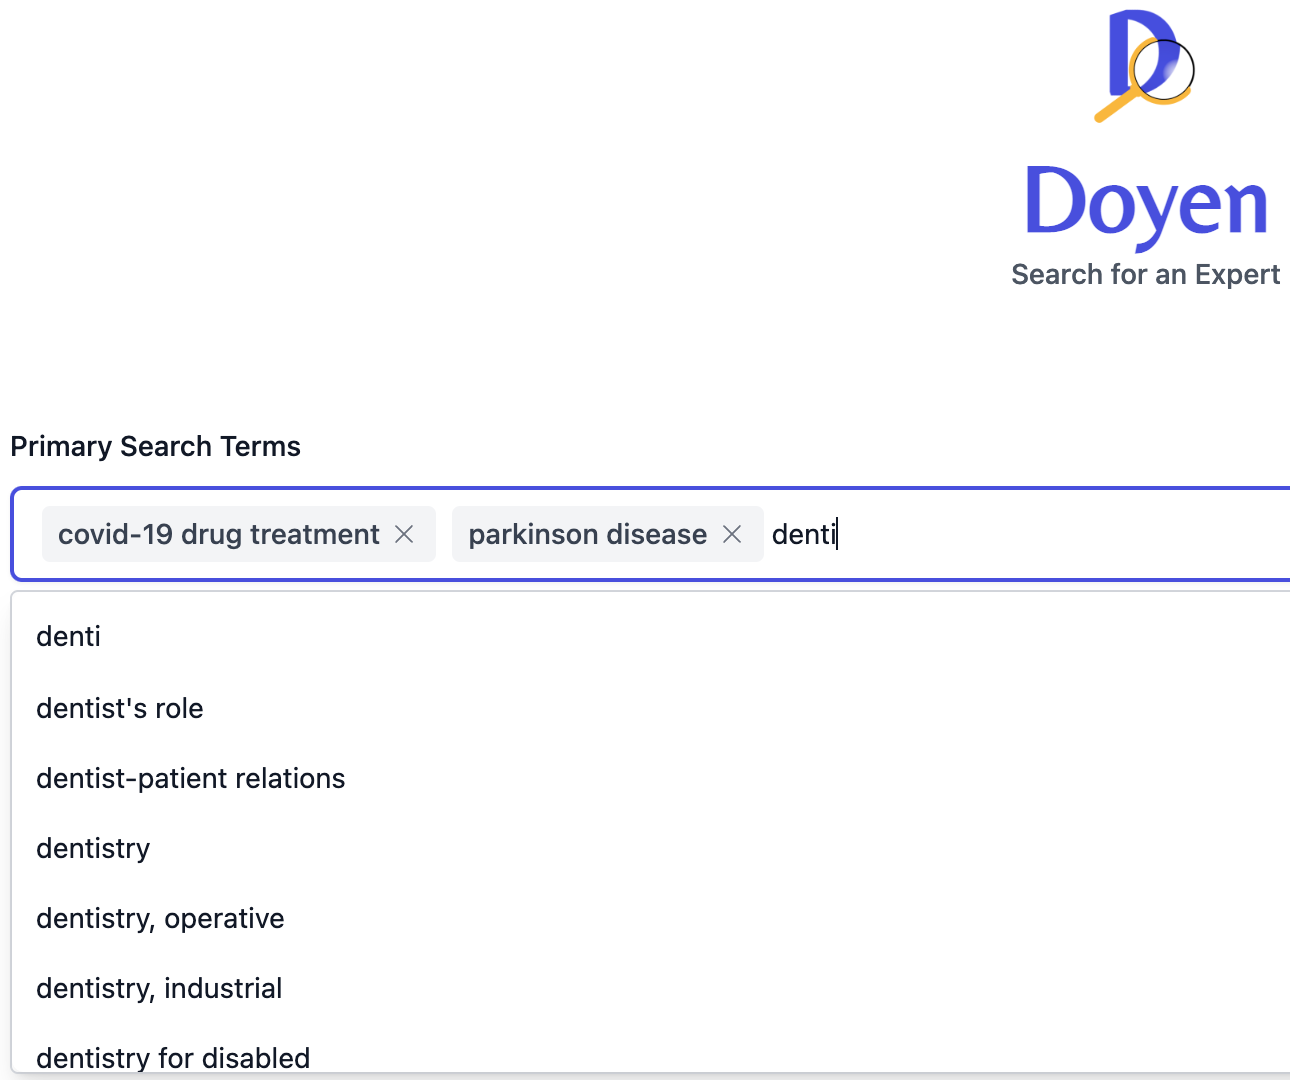
\includegraphics[width=\figwidth]{Images/ui-searchbar.png}
    \caption[Doyen App Search Bar]{\textbf{Doyen app search bar:} A view of the search bar with a user constructing a query using the autocomplete MeSH term list.}
    \label{fig:ui-searchbar}
\end{figure*}

\begin{figure*}[ht!]
    \tiny
    \centering
    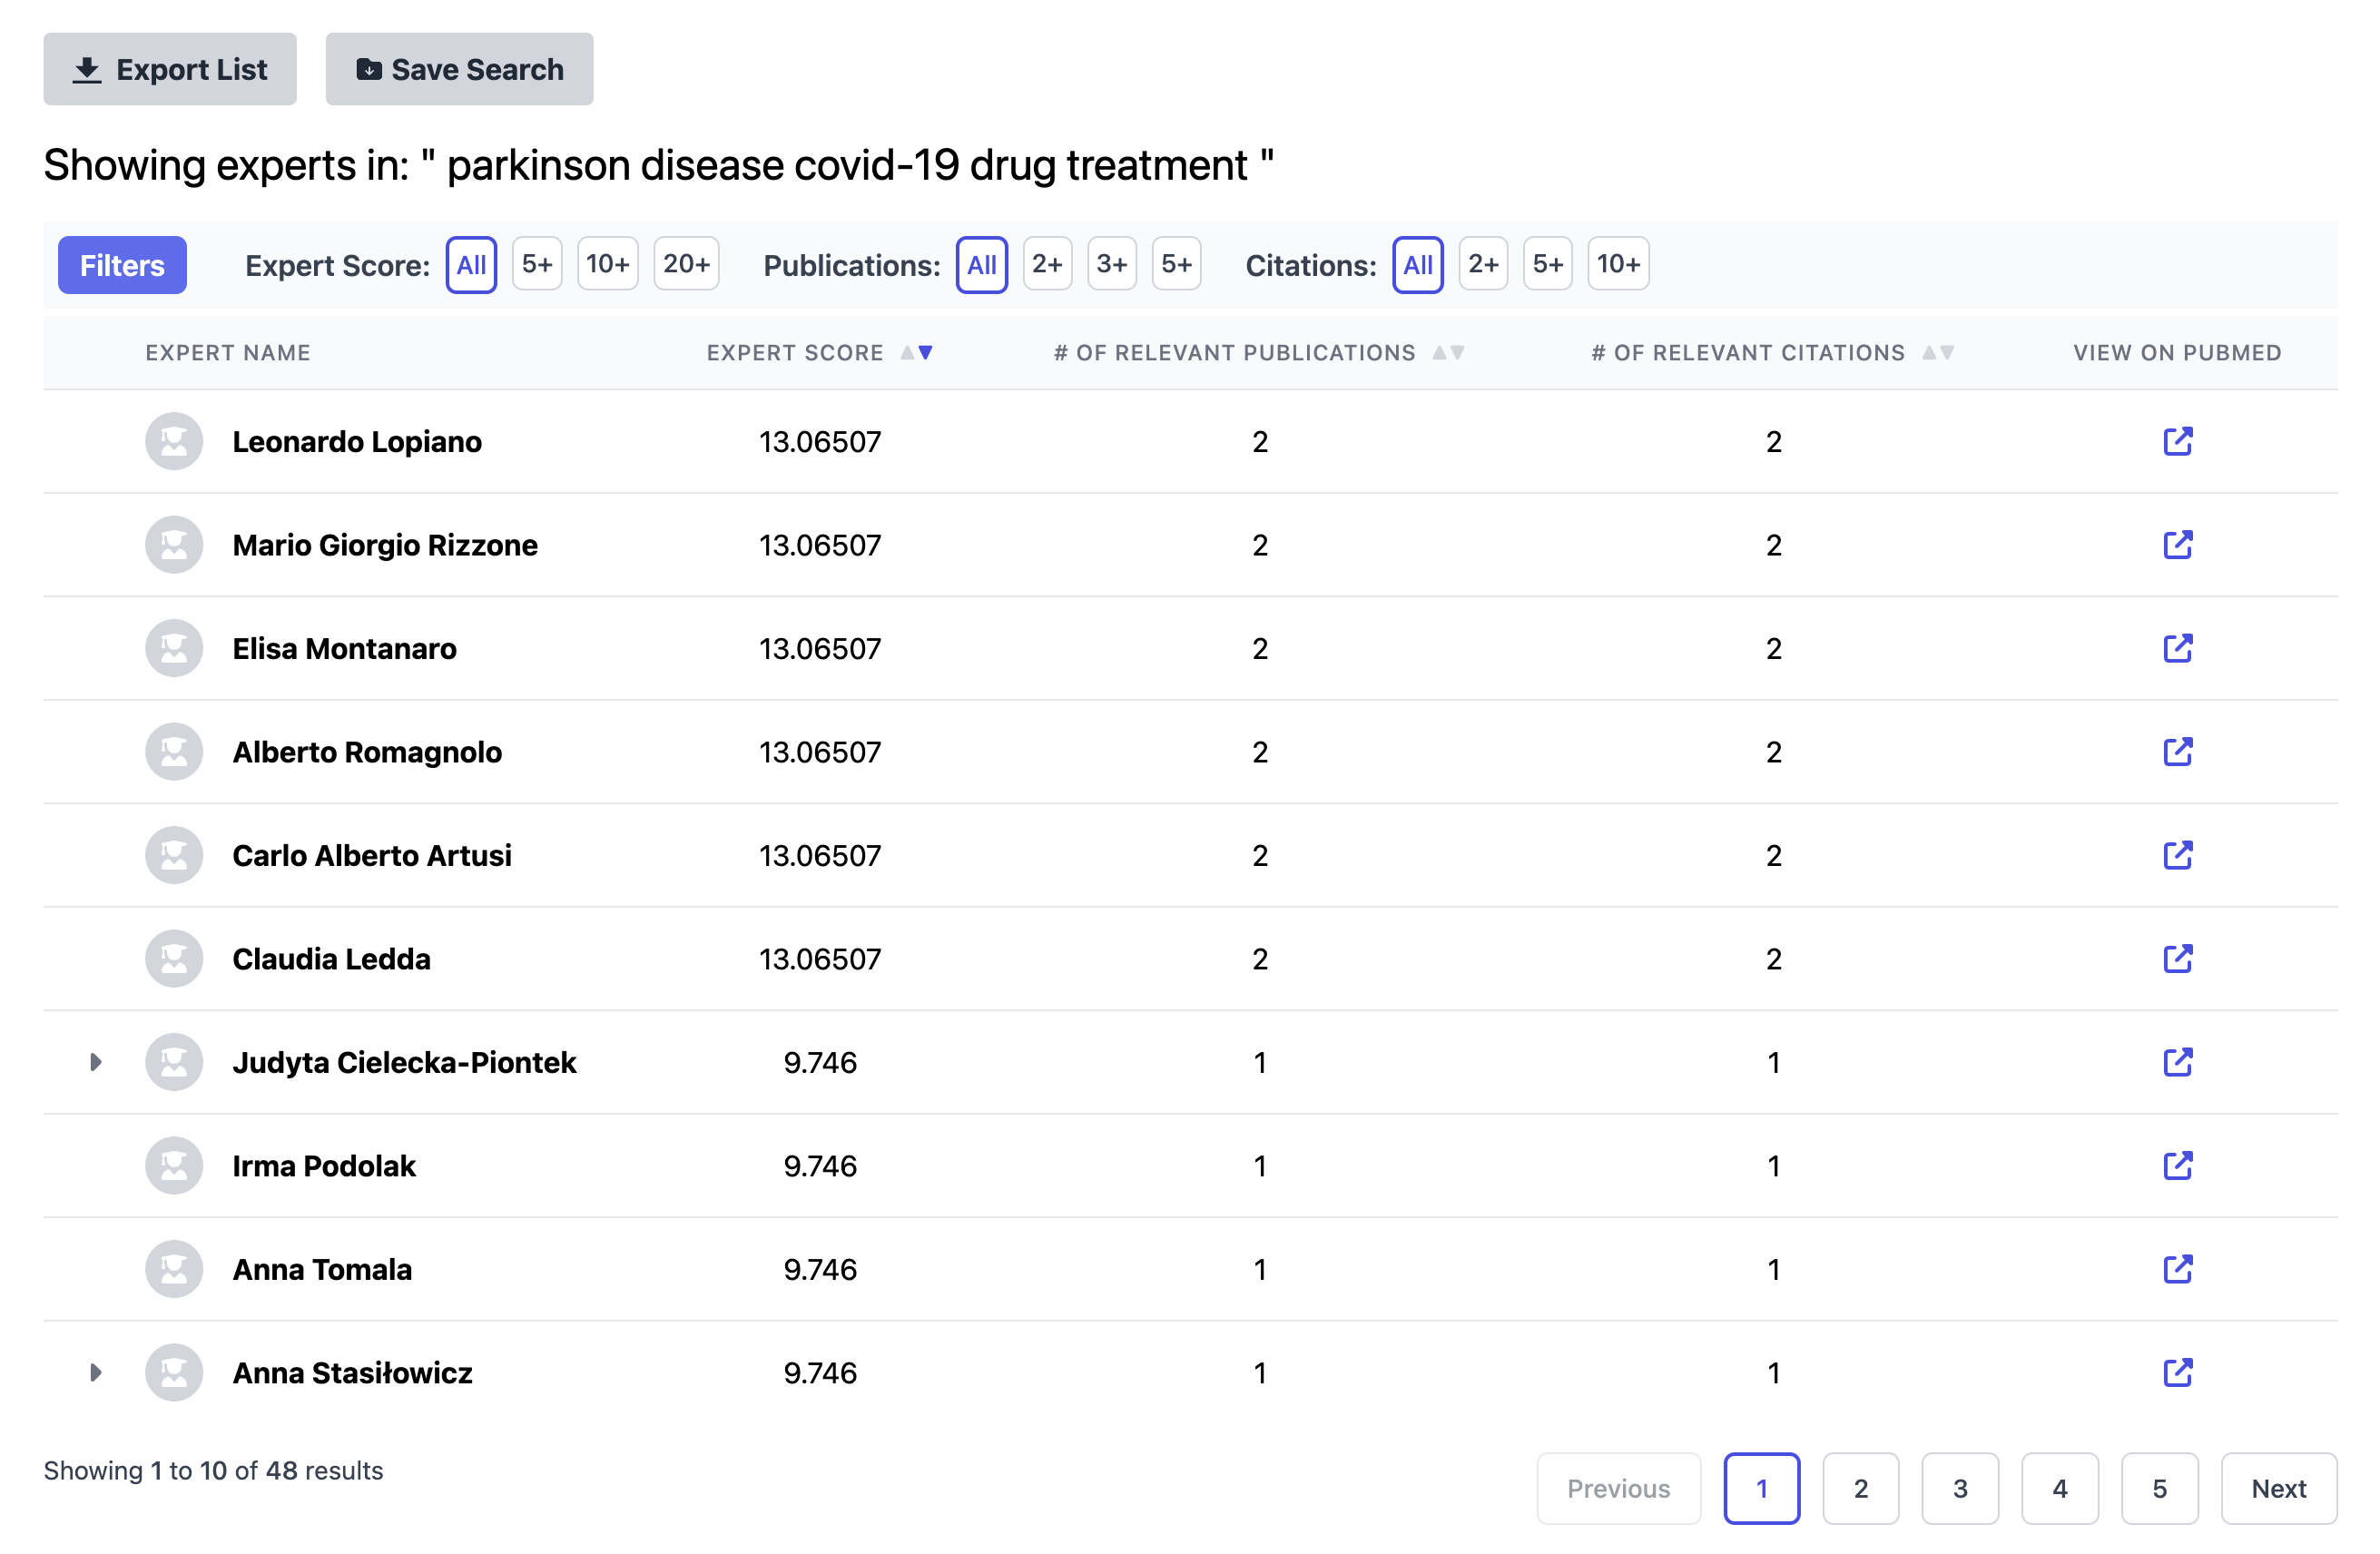
\includegraphics[width=\figwidth]{Images/ui-results.png}
    \caption[Search Results Page]{\textbf{Search results page:} A view of the results page displaying paginated expert search results, including sorting and filtering options.}
    \label{fig:ui-results}
\end{figure*}

\subsubsection{Back-End Integration and Search Results Display}

Once satisfied with their staged query, users hit ``search,'' and the search terms list is sent to Elasticsearch for a quick search of indexed PubMed publications. Elasticsearch's advantage lies in its ability to semantically search for any word in publication abstracts and titles without being restricted to MeSH terms. As shown in \autoref{fig:ui-results}, upon submitting a search query, the web application sends an API request to the back-end, which processes the query and returns a JSON object containing relevant search results. These results are then displayed on the results page, giving users an overview of the returned authors and their associated information. The interactive table presents the top 50 results sorted by the highest Relevancy Score.

\subsubsection{Filters, Sorting, and Collaborators Drop-down}

Users can sort the table based on Relevant Publication count and Relevant Citation count and filter by the number of each. The expert's section containing author identification also displays a drop-down for users to view a list of coauthors who have collaborated with the expert listed. Additionally, as shown in \autoref{fig:ui-collaborators}, users can download a PDF list of all returned authors for future reference or save their current search, allowing them to access and explore pertinent information efficiently. This functionality enhances the overall search experience provided by our web application. Users can also filter the display results by score value, publication count, and citation count and choose to view only experts with known collaborators in the drop-down list. Lastly, users can click to view relevant publications corresponding to the search directly on PubMed. 

\begin{figure*}[ht!]
    \tiny
    \centering
    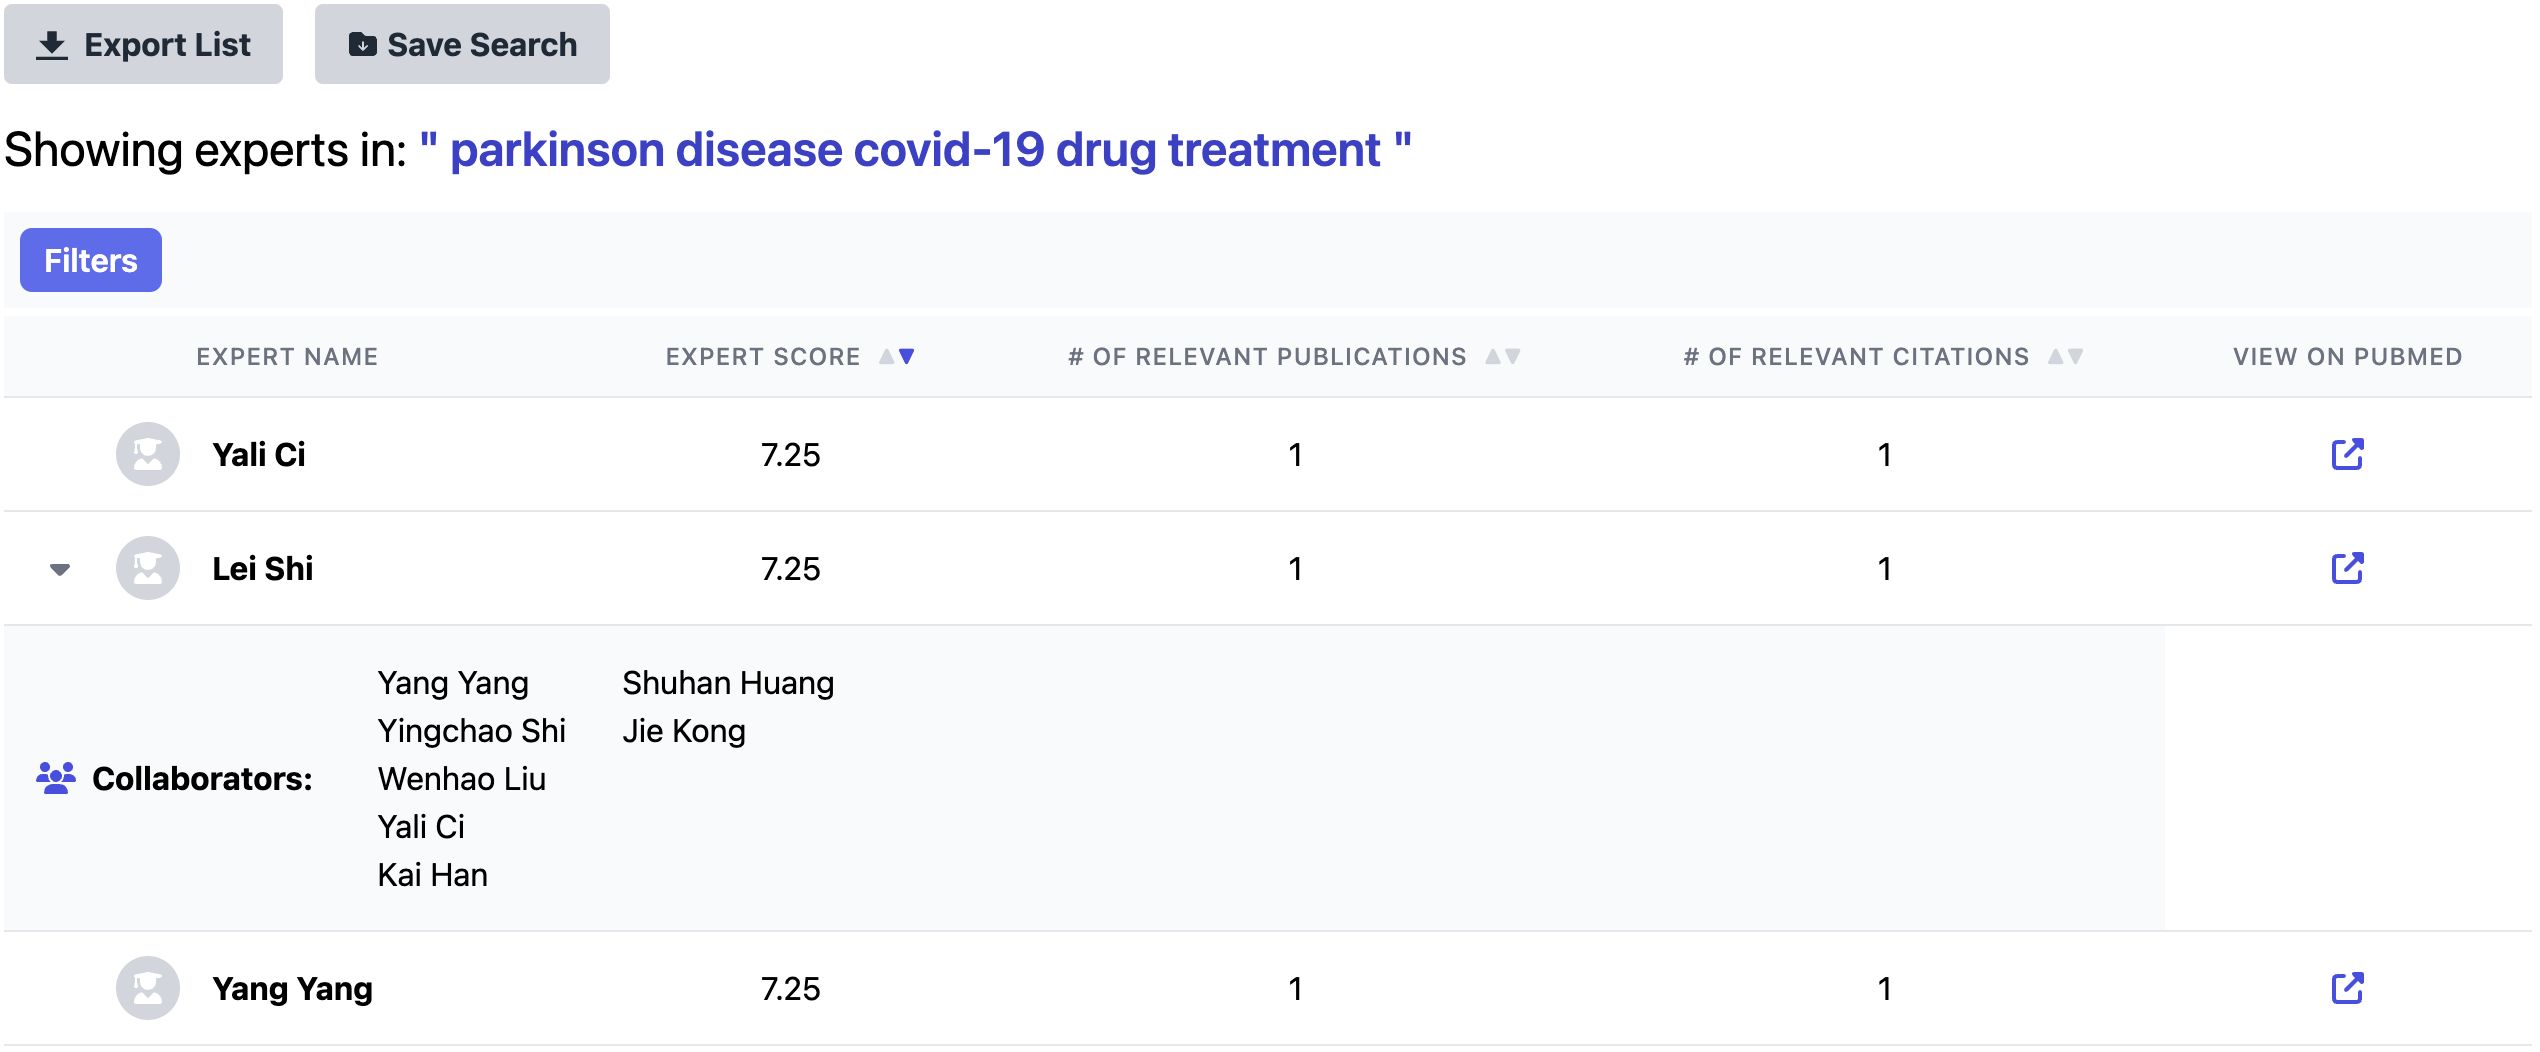
\includegraphics[width=\figwidth]{Images/ui-collaborators.png}
    \caption[Collaborators List Drop-Down]{\textbf{Collaborators list drop-down:} A view of an expert's collaborators in a displayed drop-down list.}
    \label{fig:ui-collaborators}
\end{figure*}
